\part{Referencial Teórico}

\chapter[As eclusas]{As eclusas}

Neste capítulo serão abordados conceitos a cerca das eclusas, seu funcionamento e os problemas enfrentados a cerca da eclusa de sobradinho

\section{O sistema de Eclusagem}

\subsection{Introdução ao sistema de eclusagem}

As eclusas são uma obras da engenharia hidráulica que permitem o transporte de embarcações por canais com diferenças de altitude \cite{locks_dams}. Elas funcionam como elevadores de água, permitindo que os navios subam e desçam através de um sistema de comportas.

O funcionamento de uma eclusa se baseia na gravidade. Quando um navio vai fazer o trajeto de descida por uma eclusa, a primeira porta da eclusa se abre permitindo que o navio entre. Assim que o navio entra, a porta é fechada novamente e a água é retirada até que atinja o mesmo nível do corpo d’água a jusante da eclusa. Quando atinge o mesmo nível, a segunda porta se abre e o navio pode sair.


\begin{figure}[h]
	\centering
	\label{fig:estr}
		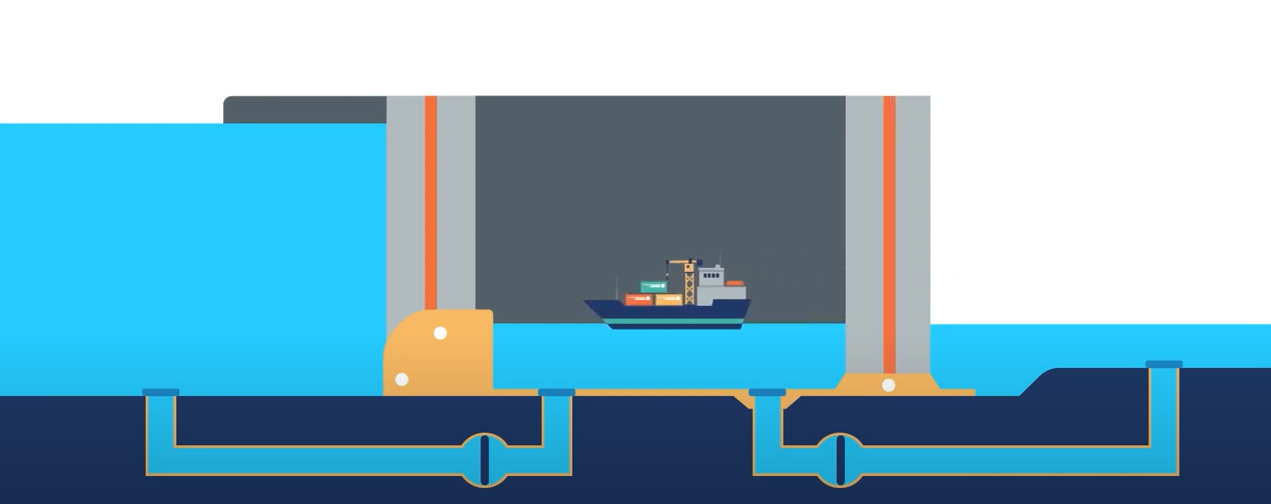
\includegraphics[keepaspectratio=true,scale=0.5]{figuras/entrada_barco.png}
	\caption{Imagem básica do processo de uma eclusa (Fonte: Acervo DNIT)}
\end{figure}

Dependendo da diferença de altitude entre o corpo d’água a montante e o corpo d’água a jusante da eclusa, ela pode ser classificada em: eclusa de baixa queda, eclusa de média queda, eclusa de alta queda e eclusa de altíssima queda. O tamanho da queda influencia em fatores importantes como a maior ou menor propensão à formação de turbulência, o tempo de enchimento e esvaziamento, variação maior ou menor no pico das vazões de enchimento/esvaziamento, problemas de cavitação, velocidade de condução nos tubos de enchimento/esvaziamento e a necessidade de sistemas mais eficientes dissipadores de energia.

As eclusas possuem um potencial econômico muito importante, pois elas permitem a navegação em rios e canais, facilitando o transporte de mercadorias e reduzindo os custos logísticos além de ser um impulso em algumas regiões do Brasil, como a região norte-nordeste, facilitando o transporte de cargas e contribuem para o crescimento econômico dessas áreas.


\subsection{A eclusa de Sobradinho}

A Eclusa de Sobradinho foi construída em 1979 e está situada no rio São Francisco. Ela é composta por uma câmara de eclusagem de 120 metros de comprimento, 17 metros de largura e 2,5 metros de calado. Essas dimensões permitem que as embarcações superem um desnível de 32,5 metros, o equivalente a um prédio de dez andares, possibilitando assim a transposição da barragem da Usina Hidrelétrica\cite{Eninfra}.

As operações na Eclusa de Sobradinho foram retomadas pelo Governo Federal, por meio do Departamento Nacional de Infraestrutura de Transportes (DNIT), em 26 de março de 2021, após terem sido interrompidas em 20181. A retomada das operações faz parte das ações executadas pelo Programa Nacional de Recuperação, Operação, Manutenção e Gestão de Eclusas (PROECLUSAS), liderado pelo DNIT.

\begin{figure}[h]
	\centering
	\label{fig:eclusasuperior}
		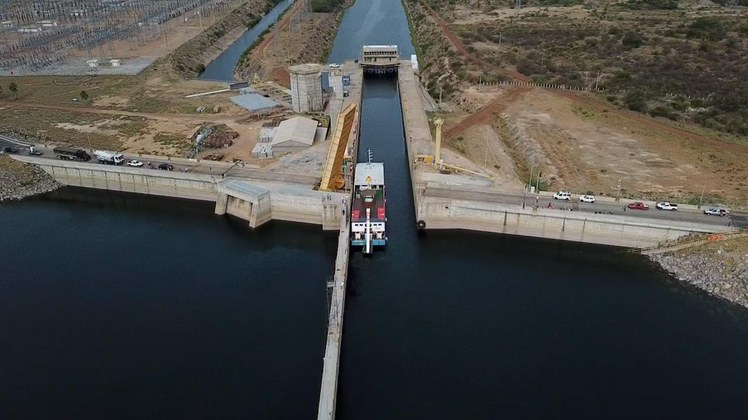
\includegraphics[keepaspectratio=true,scale=0.4]{figuras/Eclusa superior.jpeg}
	\caption{Elcusa de Sobradinho, Vista superior Fonte: (Acervo DNIT)}
\end{figure}
\begin{figure}[h]
	\centering
	\label{fig:eclusafrente}
		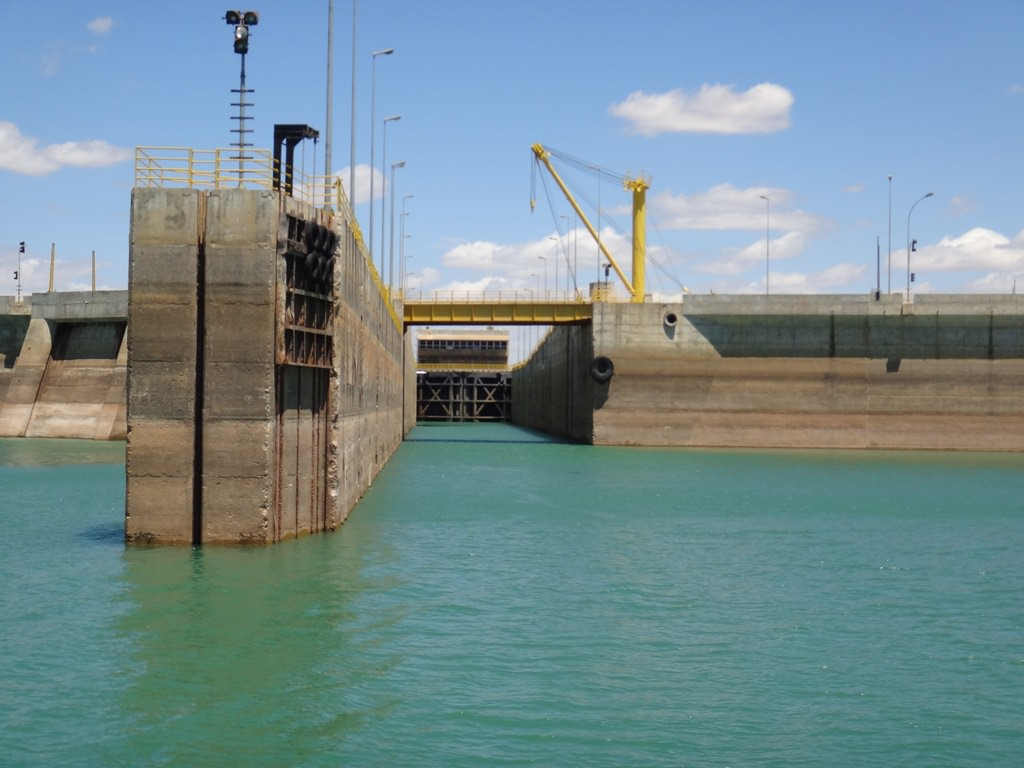
\includegraphics[keepaspectratio=true,scale=0.35]{figuras/eclusa frontal.jpg}
	\caption{Elcusa de Sobradinho, Vista frontal Fonte: (Acervo DNIT)}
\end{figure}

%\begin{figure}[h]
%	\centering
%	\label{fig:movtotal}
%		\includegraphics[keepaspectratio=true,scale=0.6]{figuras/Diagrama_movimentacao.jpg}
%	\caption{Movimento total da base com os ângulos}
%\end{figure}


\subsection{Uma Breve descrição do funcionamento das Eclusas}


Uma eclusa possui no centro as câmaras de água, que servem como grandes reservatórios fechados por comportas em ambos os lados. Essas câmaras são projetadas para acomodar as embarcações durante o processo de transposição de níveis de água. As comportas são dispositivos de controle de fluxo de água que regulam a entrada e saída de embarcações das câmaras de água. Elas também são responsáveis por manter o nível de água adequado dentro da eclusa durante a eclusagem.

Os sistemas de controle desempenham um papel fundamental no funcionamento da eclusa, monitorando e coordenando todas as operações relacionadas à sua operação. Isso inclui o acionamento das comportas, o controle dos sistemas de enchimento e esvaziamento das câmaras de água e a comunicação com as embarcações durante o processo de eclusagem.

Além disso, as eclusas são equipadas com dispositivos de ancoragem e amortecimento para garantir a segurança das embarcações durante a eclusagem. Esses dispositivos ajudam a evitar colisões e danos às embarcações e à própria estrutura da eclusa.

O processo de eclusagem é complexo e envolve três fases: A primeira fase (Fig.\ref{fig:primeirafase}) envolve a entrada das embarcações na câmara de água da eclusa e as comportas são fechadas atrás delas para garantir a estanqueidade da câmara. Na segunda fase(Fig.\ref{fig:segundafase}), o nível de água na câmara de água é ajustado para igualar o nível da água com o trecho de água a ser alcançado. Já na terceira fase, uma vez que o nível de água é ajustado, as comportas na extremidade oposta da eclusa são abertas e a embarcação pode sair para o trecho de água de nível diferente \cite{Eninfra}.


\begin{figure}[h]
	\centering
	\label{fig:primeirafase}
		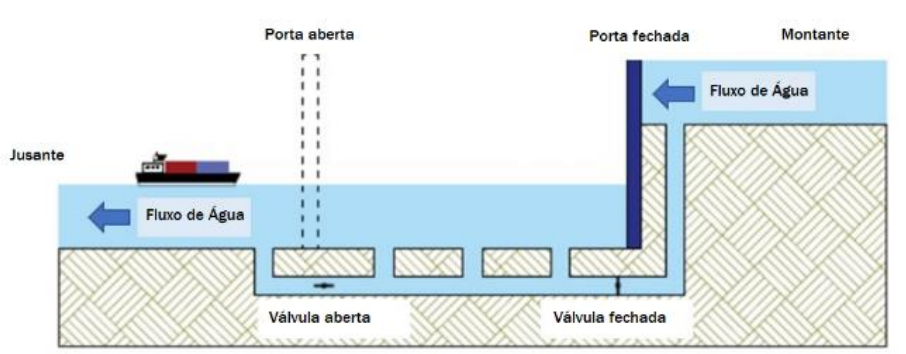
\includegraphics[keepaspectratio=true,scale=0.6]{figuras/fase01.png}
	\caption{Primeira Fase: Entrada da embarcação na eclusa Fonte: (Acervo DAQ)}
\end{figure}

\begin{figure}[h]
	\centering
	\label{fig:segundafase}
		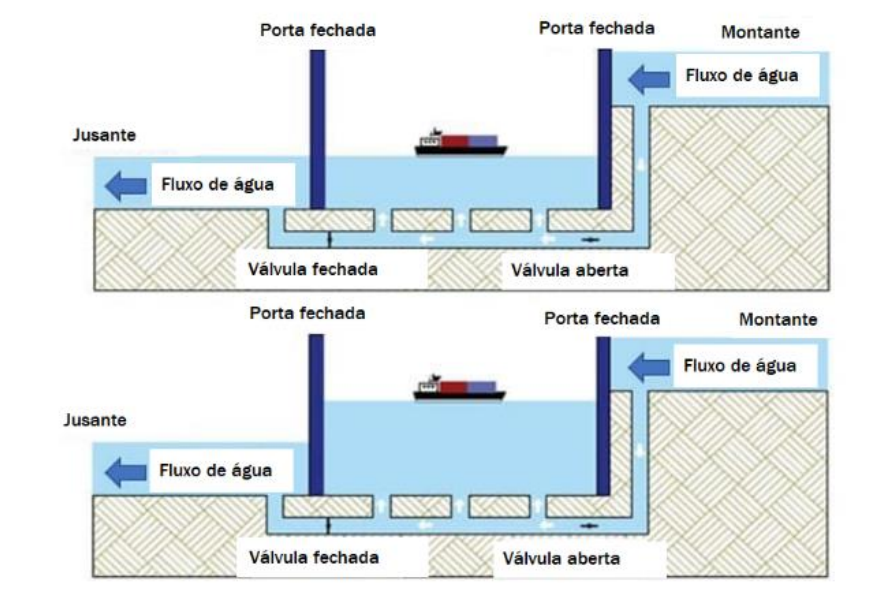
\includegraphics[keepaspectratio=true,scale=0.6]{figuras/fase02.png}
	\caption{Segunda Fase: Entrada da embarcação na eclusa Fonte: (Acervo DAQ)}
\end{figure}

\begin{figure}[h]
	\centering
	\label{fig:terceira fase}
		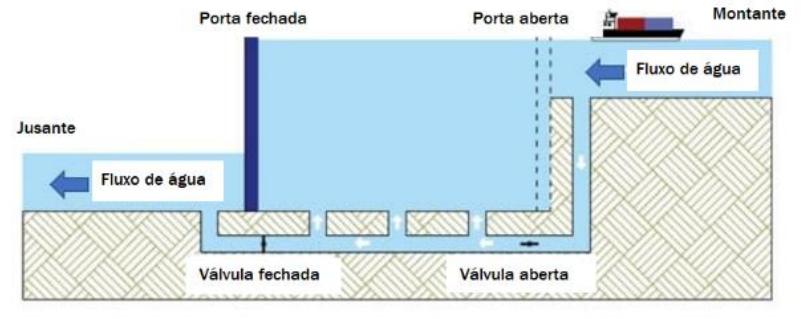
\includegraphics[keepaspectratio=true,scale=0.6]{figuras/fase03.png}
	\caption{Primeira Fase: Entrada da embarcação na eclusa Fonte: (Acervo DAQ)}
\end{figure}

\section{Automação de uma Eclusa}

\subsection{Uma introdução sobre Automação Industrial}

A automação industrial é um campo de estudo em constante evolução que se concentra na aplicação de tecnologias avançadas para otimizar processos industriais. Ela desempenha um papel crucial na melhoria da eficiência, segurança e produtividade nas indústrias modernas\cite{Groover}.

A automação industrial é a utilização de sistemas de controle, como computadores ou robôs, e tecnologias de informação para lidar com diferentes processos e máquinas em uma indústria para substituir um humano. Ela é vital para muitas indústrias, incluindo manufatura, transporte, serviços públicos, defesa, energia, e saúde.

Suas vantagens consiste em vários benefícios, incluindo aumento da produtividade, melhoria da qualidade, redução de custos, e melhoria da segurança no local de trabalho. Além disso, ela permite que as empresas se mantenham competitivas em um mercado global cada vez mais competitivo.

\subsection{Componentes de uma eclusa}

\begin{itemize}
	\item Controlador Lógico Programável (CLP): O CLP é um computador compacto de alta robustez com o objetivo de uso em Indústria, que tem a função de executar as linhas dos diagramas Ladder, permanecendo como elemento principal de controle do sistema da eclusa.
	\item Sistema Supervisório (SCADA): Este é um software usado para controlar processos industriais à distância. Ele permite aos operadores visualizar e interagir com o estado operacional da eclusa.
	\item Sensores e Atuadores: Os sensores são usados para coletar dados do ambiente, como nível de água, posição das portas, etc. Os atuadores, como motores e válvulas, realizam ações físicas baseadas nas instruções do CLP.	
    \item Redes de Comunicação Industrial: Estas redes permitem a comunicação entre o CLP, o sistema supervisório e os vários sensores e atuadores, na eclusa se usa o protocolo \textit{Modbus}.
    \item Sistema de CFTV: Um sistema de Circuito Fechado de Televisão (CFTV) é utilizado para acompanhamento de eclusagens.
\end{itemize}

\section{Modelagem matemática do sistema de uma eclusa}

Consideramos o fluxo de água ao longo da comporta (Figura \ref{fig:modelagem}), e podemos assumir o sistema como três reservatórios: um reservatório a montante, um reservatório a jusante e um reservatório na câmara de eclusagem. Existe também duas comportas, onde conectam os reservatórios da montante e da jusante a câmara de eclusagem. Em cada comporta (Que para o exemplo será modelada como uma válvula de restrição) temos uma resistência de restrição $R$ dada por:

\begin{equation} \label{eq:resistencia_teoria1}
 R=\frac{\mathrm{d} H }{\mathrm{d} Q}
\end{equation}

Onde:

    $H$: Variação da altura, em metros ($m$)
    $Q$: Variação da vazão em volume, em metros cúbicos por segundo ($m^3/s$)

Em todos os reservatórios, temos uma capacitância, que é dada por:

\begin{equation} \label{eq:capacitancia_teoria1}
 C=\frac{\mathrm{d} L }{\mathrm{d} H}
\end{equation}

Onde:

    $L$: Variação da quantidade de líquido armazenado, em metros cúbicos ($m^3$)
    $H$: Variação da altura, em metros ($m$)

Podemos fazer uma modelagem de acordo com \cite{Ogata} sendo $Q'$ a vazão em regime permanente, em metros ($m^3/s$), $q_1$ e $q_0$ pequenas variações das vazões de entrada e saída, $H'$ a altura do nível e $h$ um pequeno desvio de nível a partir do seu valor em regime permanente.

Então, se considerarmos apenas a abertura de comportas entre montante e câmara de eclusagem, e jusante e câmara de eclusagem e que temos uma variação da altura e do fluxo ao longo do tempo, temos a seguinte sistema de equação diferencial \cite{Ogata}:

\begin{equation} \label{eq:eqdif1}
 RC\frac{dh}{dt}+h=Rq_i
\end{equation}

observando que $RC$ é a constante de tempo do sistema. Fazendo a transformada de Laplace, temos que a razão $H(s)$ e $Q_i(s)$ é:

\begin{equation} \label{eq:laplace1}
 \frac{H(s)}{Q_i(s)}=\frac{R}{RCs+1}
\end{equation}

Com isso, podemos admitir que a razão entre a entrada e a saída do fluxo podemos retirar a função de transferência sendo:

\begin{equation} \label{eq:laplace2}
 \frac{Q_0(s)}{Q_i(s)}=\frac{1}{RCs+1}
\end{equation}

Apesar de  \ref{eq:laplace2} ser a modelagem básica do sistema, o sistema Montante - Câmara de Eclusagem - Jusante é um sistema de nível que possui mais de uma interação. Então de acordo com \cite{Ogata}, temos que para um fluxo $q_k$ da câmara de eclusagem, $R_k$ e $C_k$ resistência e capacitância da câmara , $q1$ o fluxo da jusante e $q2$ o fluxo da montante, Então o resultado é a seguinte função de transferência:

\begin{equation} \label{eq:functransf1}
\frac{Q_1(s)}{Q_k(s)}=\frac{1}{R_kC_kR_1C_1s^2+(R_1C_1+R_kC_k+R_1Ck)s+1}
\end{equation}

e

\begin{equation} \label{eq:functransf2}
\frac{Q_2(s)}{Q_k(s)}=\frac{1}{R_kC_kR_2C_2s^2+(R_2C_2+R_kC_k+R_2Ck)s+1}
\end{equation}

Com \ref{eq:functransf1} e \ref{eq:functransf2} podemos retirar a função de transferência entre montante e jusante, dada por


\begin{equation} \label{eq:functransf2}
\frac{Q_2(s)}{Q_1(s)}=\frac{R_1C_1+R_1}{R_2C_2+R_2} = \frac{\tau _1}{\tau _2} + \frac{R_1}{R_2}
\end{equation}

onde $\tau _1$ e $\tau _2$ São as constantes de tempo de jusante e montante

\begin{figure}[h]
	\centering
	\label{fig:modelagem}
		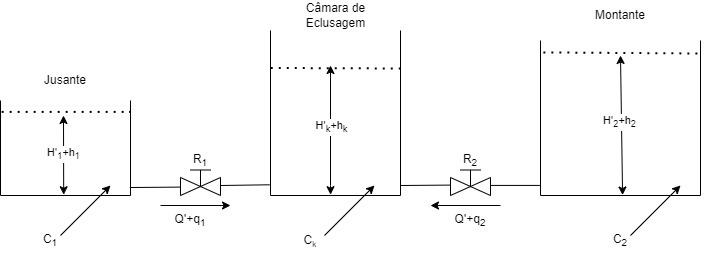
\includegraphics[keepaspectratio=true,scale=0.6]{figuras/modelagem.jpg}
	\caption{Modelo básico de modelagem de uma eclusa}
\end{figure}

%https://easytromlabs.com/arduino/arduino-lab-11-controle-de-angulo-de-fase-para-uma-carga-indutiva-e-resistiva-parte-1/?print=print

\section{Motores e bombas industriais}

No cenário industrial moderno, bombas e motores desempenham um papel crucial em diversas aplicações, desde o fornecimento de água até processos de manufatura complexos. Eles são essenciais para o funcionamento eficiente de sistemas de produção, transporte de fluidos e manuseio de materiais.

No que abrange os motores temos os Motores Trifásicos que são os mais comuns em aplicações industriais devido à sua robustez, eficiência e baixo custo de manutenção. O seu funcionamento é baseado baseados no princípio de indução eletromagnética, onde a corrente elétrica induzida no rotor é responsável por criar torque, Motores Monofásicos que são Utilizados em aplicações de menor potência onde a rede elétrica disponível é monofásica. Embora menos eficientes que os trifásicos, são adequados para pequenos equipamentos e ferramentas.  

De acordo com \cite{chapman}, os motores de indução trifásicos operam baseados no campo magnético girante criado pela corrente trifásica no estator. Este campo induz uma corrente no rotor, que interage com o campo magnético para produzir torque. A velocidade do motor é determinada pela frequência da corrente alternada e o número de polos do motor.

\begin{figure}[h]
	\centering
	\label{fig:bombas}
		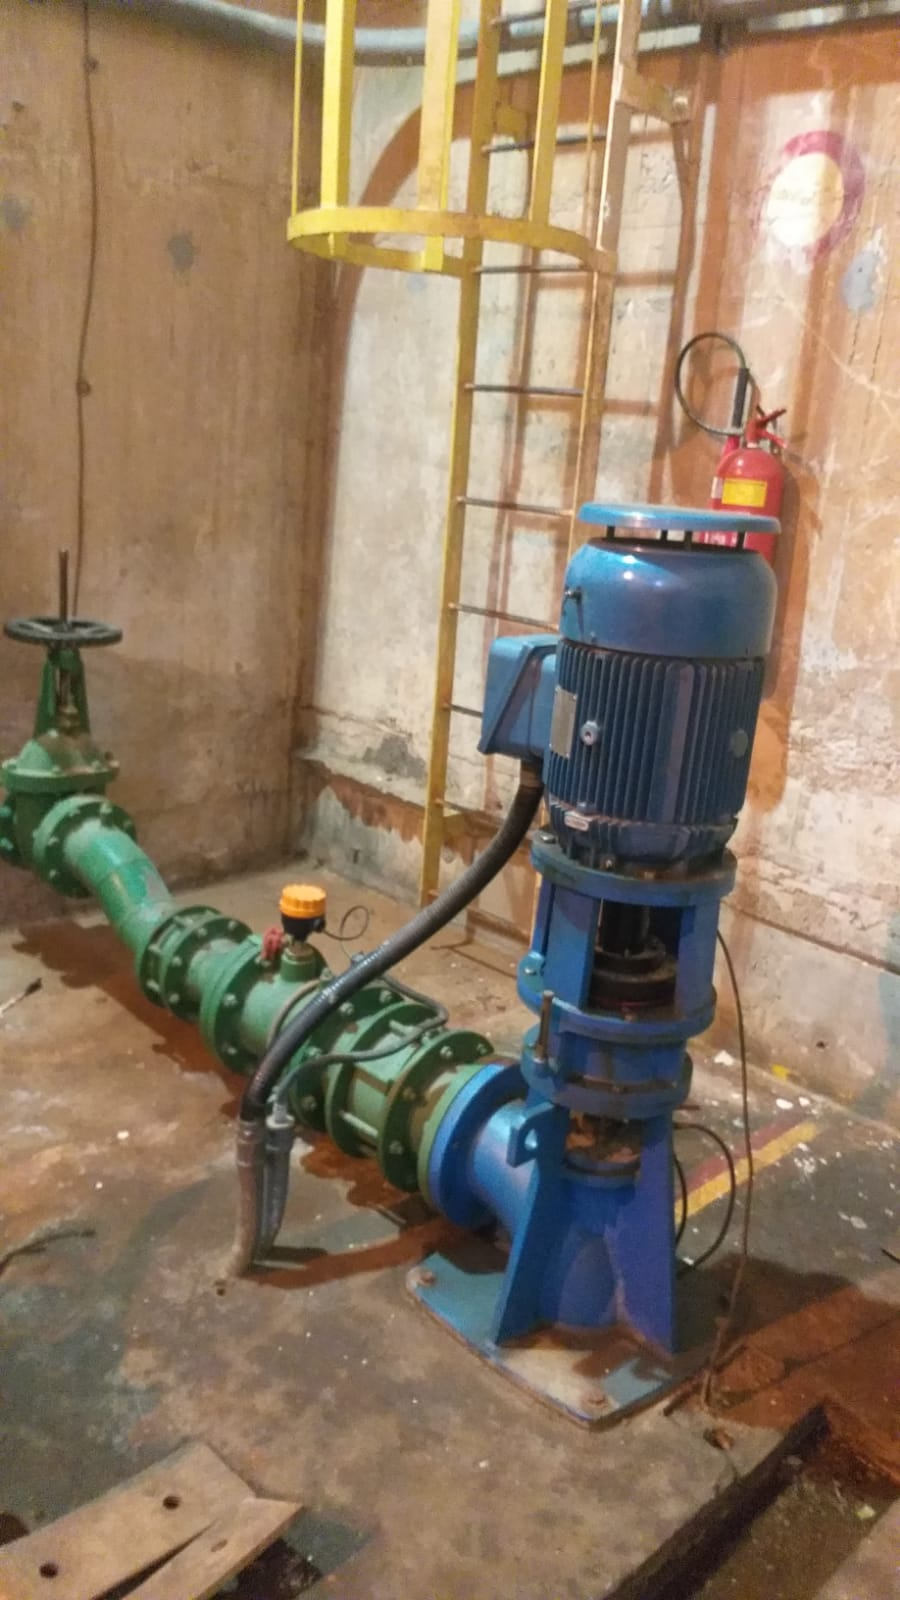
\includegraphics[keepaspectratio=true,scale=0.15]{figuras/bomba.jpeg}
	\caption{bomba usada para adução e escoamento dos poços}
\end{figure}


Segundo \cite {Groover}, A integração de bombas e motores com sistemas de automação e controle é importante para a para otimizar a eficiência energética, reduzir custos operacionais e melhorar a confiabilidade dos processos industriais. Tecnologias como inversores de frequência (VFDs) permitem o controle preciso da velocidade de motores, adaptando-se às necessidades do processo em tempo real. Sensores e CLPs monitoram parâmetros críticos, ajustando automaticamente as operações para maximizar a eficiência e minimizar o desgaste dos equipamentos.


\section{Inversores de Frequência}

\cite {hashid} define inversores de frequência, também conhecidos como drives de frequência variável (VFDs), como dispositivos eletrônicos utilizados para controlar a velocidade e o torque de motores elétricos AC. Eles convertem a tensão de entrada fixa e a frequência da rede elétrica em uma saída de tensão e frequência variável, permitindo um controle preciso do motor.

Como princípio de funcionamento, segundo \cite {hashid} Os inversores de frequência operam em três estágios principais: Retificação: A corrente alternada da rede elétrica é convertida em corrente contínua através de um retificador. Filtragem: A corrente contínua é suavizada por capacitores e indutores para eliminar ondulações. Inversão: A corrente contínua é convertida de volta em corrente alternada com a frequência e tensão desejadas por meio de um inversor, que utiliza dispositivos de comutação eletrônica como IGBTs (\textit{Insulated Gate Bipolar Transistors}).

\begin{figure}[h]
	\centering
	\label{fig:modelagem}
		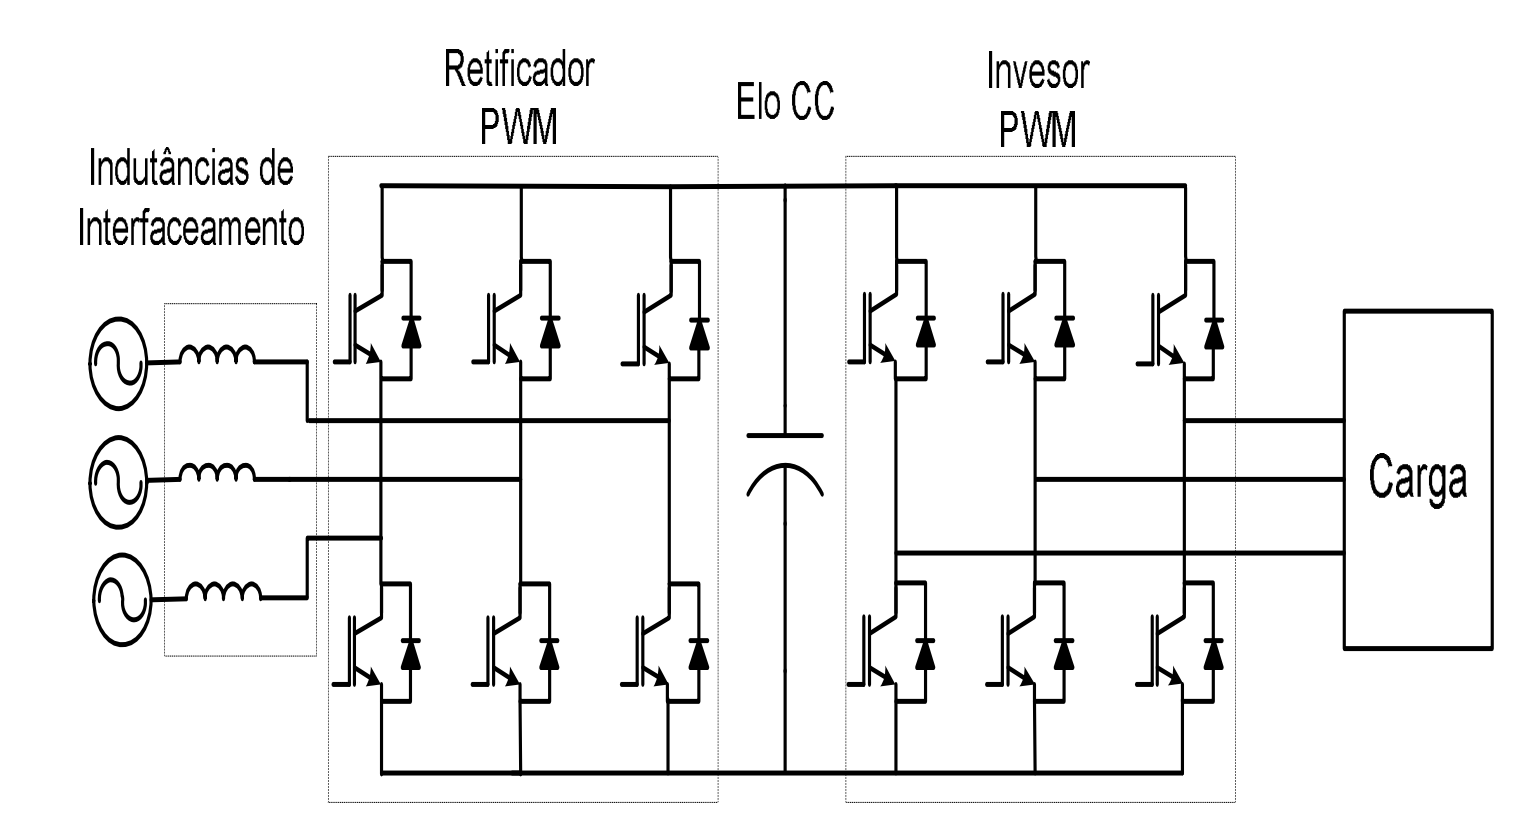
\includegraphics[keepaspectratio=true,scale=0.3]{figuras/inversor.png}
	\caption{Funcionamento básico de um inversor. Fonte: \cite{SBA}}
\end{figure}

Os benefícios dos Inversores são em suma a Eficiência Energética, Permitindo ajustar a velocidade do motor conforme a demanda do processo, reduzindo o consumo de energia. O Controle Preciso, proporcionando um controle mais preciso da velocidade e do torque do motor, melhorando a qualidade do processo. A proteção do Equipamento, incluindo diversas proteções contra sobrecorrente, sobretensão, sobretemperatura, e inversão de fase, prolongando a vida útil do motor e do sistema e a
redução de desgaste, sendo a partida suave e o controle de aceleração/desaceleração reduzindo o desgaste mecânico.

Inversores são amplamente utilizados em diversas indústrias, incluindo controle de velocidade de motores em linhas de produção, HVAC , controle de bombas e ventiladores para eficiência energética, Controle de bombas em estações de tratamento, Controle de guindastes, elevadores e transportadores.

\section{Protocolo de Comunicação Modbus}

De acoro com \cite{modbus2006}, o protocolo Modbus TCP é uma variante do protocolo Modbus original, desenvolvido pela Modicon (agora \textit{Schneider Electric}) em 1979 para comunicação entre CLPs. Adaptado para operar sobre redes \textit{Ethernet} utilizando o protocolo TCP/IP, o Modbus TCP tornou-se amplamente utilizado na automação industrial devido à sua simplicidade e eficácia na comunicação entre dispositivos heterogêneos.

O Modbus TCP tem funcionamento em três camadas principais dentro de um modelo  Referência para Interconexão de Sistemas Abertos (OSI), a Camada de Aplicação, onde temos a  Unidade de Dados do Protocolo (PDU) que Consiste em um cabeçalho e os dados e as Funções Modbus, que são instruções específicas para leitura/escrita de registradores e bobinas, assim como funções de diagnóstico.
Em segundo temos a Camada de Transporte, onde o Modbus TCP utiliza o protocolo de transporte TCP, que garante a entrega confiabilidade a entrega de dados e por ultimo a Camada de Rede, onde fornce a via ethernet a interconexão física e a camada de enlace de dados para os dispositivos na rede local.


Segundo a documentação de \cite{modbus2006} Um pacote Modbus TCP ou mesmo RTU possui 8 bytes como identificador, sendo 7bytes de  Cabeçalho MBAP (\textit{Modbus Application Protocol Header}), e desses 7 bytes, 2 bytes são de Identificador de Transação, que são Associados a requisição e resposta. 2 bytes de Identificador de Protocolo, sendo sempre 0 para Modbus. 2 bytes de Comprimento, que indica o tamanho dos dados subsequentes e 1 byte de Identificador de Unidade que Identifica o dispositivo de destino.

O ultimo byte é dedicado ao PDU (\textit{Protocol Data Unit}), que possui vários tipos de Código de Função, que identifica e Indica a função a ser executada (por exemplo, leitura, escrita).
Os principais dados enviados pelo protocolo são:

\begin{itemize}
	\item 0x01 (Leitura de Bobinas): Leitura do estado das bobinas (saídas digitais).
	\item 0x02 (Leitura de Entradas Discretas): Leitura do estado das entradas discretas.
	\item 0x03 (Leitura de Registradores de Retenção): Leitura dos registradores de armazenamento.
    \item 0x04 (Leitura de Registradores de Entrada): Leitura dos registradores de entrada.
    \item 0x05 (Escrita em Única Bobina): Escrita no estado de uma bobina.
    \item 0x06 (Escrita em Único Registrador): Escrita em um único registrador.
    \item 0x0F (Escrita em Múltiplas Bobinas): Escrita no estado de múltiplas bobinas.
    \item 0x10 (Escrita em Múltiplos Registradores): Escrita em múltiplos registradores.
\end{itemize}

O Modbus TCP oferece diversas vantagens, dentre as quais a facilidade de comunicação entre diversos componentes e fabricantes, não causar problemas nas diversas arquiteturas de rede, a maior facilidade entre interfaces humano-maquina e sistemas de supervisório.

\section{Conversores Analógico/Digital}

Os conversores Analógico-Digital (A/D) são componentes essenciais em sistemas de aquisição de dados, permitindo a conversão de sinais analógicos contínuos em dados digitais discretos que podem ser processados por microcontroladores e sistemas de processamento digital. 

A quantização é o processo de mapeamento de um sinal analógico contínuo para valores digitais discretos. Este processo introduz um erro chamado erro de quantização, que é a diferença entre o valor analógico real e o valor quantizado. O sinal analógico é dividido em intervalos de amplitude iguais Cada intervalo é representado por um valor digital específico, sendo um conversor A/D com \( N \) bits pode representar \( 2^N \) níveis distintos.

A quantização de um valor de entrada \( V_{in} \) para um nível digital \(Q(V_{in})\) pode ser expressa como \cite{ieee_adc}:

\begin{equation} \label{eq:ad1}
Q(V_{in}) = \Delta V \cdot \left\lfloor \frac{V_{in}}{\Delta V} + 0.5 \right\rfloor
\end{equation}

Onde \( \Delta V \) é a resolução do conversor A/D.

O erro de quantização é dado pela diferença entre o valor analógico real \( V_{in} \) e o valor quantizado \( Q(V_{in}) \) \cite{ieee_adc}::
\begin{equation} \label{eq:ad2}
e_q = V_{in} - Q(V_{in})
\end{equation}

Já a resolução em nível de tensão (\( \Delta V \)) é dada pela relação entre o intervalo de entrada total (\( V_{ref} \)) e o número de níveis distintos\cite{ieee_adc}::
\begin{equation} \label{eq:ad3}
\Delta V = \frac{V_{ref}}{2^N}
\end{equation}

É importante analisar que em um conversor A/D, além do processo de quantização, de erro e resolução, segundo \cite{ieee_adc}, os principais parâmetros de avaliação para a caracterização de um conversor A/D são a Relação Sinal- Ruído (SNR), a relação sinal-ruído e distorção (SINAD), o número efetivo de bits (ENOB), a distorção harmônica total (THD) e o intervalo dinâmico livre de componentes espúrias (SFRD).

O SNR (Signal-to-Noise Ratio) é uma métrica que descreve a relação entre o nível do sinal e o nível do ruído em um conversor A/D. É uma medida importante da qualidade do sinal digitalizado.

Para um conversor ideal, o SNR é dado por:
\begin{equation} \label{eq:SNR}
SNR= 6,02N + 1,76dB
\end{equation}
onde \( N \) é o número de bits do conversor.

A Relação Sinal-Ruído e Distorção (SINAD) é uma métrica que inclui todos os componentes de ruído e distorção presentes no sinal. Ela é usada para avaliar a qualidade de um conversor A/D, considerando não apenas o ruído, mas também as distorções harmônicas, ela é definida como\cite{ieee_adc}:

\begin{equation}\label{eq:SINAD}
SINAD_{dB} = 20 \times \log_{10} \left( \frac{S}{\sqrt{\sum_{f \ne f_{in}} S_i^2}} \right)
\end{equation}

onde \( S \) é a potência do sinal útil e $\sum_{f \ne f_{in}} S_i^2$ é a soma da potência do ruído e das distorções harmônicas.

O ENOB (Effective Number of Bits) é uma métrica que representa a resolução efetiva de um conversor A/D, levando em conta os efeitos do ruído e de outros erros \cite{ieee_adc}:.

O ENOB é calculado a partir do SNR real medido do sistema:
\begin{equation} \label{eq:ENOB}
ENOB = \frac{SINAD_{dB} - 1,76}{6,02}
\end{equation}

O ENOB fornece uma medida mais realista da performance do conversor, refletindo a resolução efetiva que pode ser alcançada na presença de ruído e distorções.

A Distorção Harmônica Total (THD) é uma métrica que quantifica a soma das potências de todas as componentes harmônicas de um sinal em relação à potência da componente fundamental.

\begin{equation} \label{eq:THD}
THD_{dB} = 20 \times \log_{10} \left( \frac{\sqrt{\sum_{i=2}^{\infty} S_i^2}}{S_1} \right)
\end{equation}

Onde \( S_{1} \) é a potência do sinal útil e \( S_{i} \) é a soma da potência do ruído e das distorções harmônicas. Um THD mais baixo indica que o sinal tem menos distorções harmônicas.

O Intervalo Dinâmico Livre de Espúrios (SFDR) é uma métrica que quantifica a faixa dinâmica de um conversor A/D, considerando o maior tom espúrio presente no sinal. O SFDR é definido como a razão entre a potência da componente fundamental e a potência do maior tom espúrio, expressa em decibéis:

\begin{equation} \label{eq:SFDR}
SFDR_{dB} = 20 \times \log_{10} \left( \frac{S_1}{S_{espurios}} \right)
\end{equation}

Os principais tipos de conversores A/D no mercado são o por Aproximação Sucessiva (SAR), O sigma-delta ($\Sigma$-$\Delta$), o Fash e o Rampa-Dupla

O SAR é um tipo de conversor A/D que opera de maneira iterativa. Ele utiliza um Conversor Digital-Analógico (DAC) interno para gerar um sinal analógico a partir de um valor digital. Este sinal é então comparado com o sinal de entrada. O processo é realizado bit a bit, começando pelo bit mais significativo (MSB) e indo até o bit menos significativo (LSB).

Em sua inicialização  O bit mais significativo (MSB) do registrador SAR é definido como 1.logo após, O valor binário atual no registrador SAR é convertido para uma tensão analógica pelo DAC. Esta tensão é então comparada com a tensão do sinal de entrada.  Se a tensão do DAC for maior que a tensão de entrada, o bit atual do registrador é definido como 0. Caso contrário, o bit permanece como 1. O processo é repetido para o próximo bit menos significativo até que todos os bits no registrador tenham sido testados. Após todos os bits serem testados, o valor no registrador SAR é a representação digital do sinal analógico de entrada. Este método é eficiente e rápido, pois o número de iterações é igual ao número de bits de resolução do conversor, tornando o tempo de conversão previsível. Além disso, os conversores SAR são amplamente utilizados devido à sua simplicidade relativa e desempenho adequado para muitas aplicações

Os conversores A/D Sigma-Delta são uma classe de conversores analógico-digital que utilizam a técnica de oversampling para obter alta resolução. Eles são amplamente utilizados em aplicações que requerem alta precisão, como medições científicas, instrumentação médica e áudio digital \cite{sigma_delta}.

Seu processo consiste em integração, onde a tensão de entrada analógica é integrada durante um certo tempo. A Quantização,onde a parte analógica do conversor é responsável pela quantização e modulação do sinal de entrada  O conversor Sigma-Delta utiliza o princípio da realimentação do sinal quantizado. Isso resulta em um filtro passa-baixas para o sinal e passa-altas para o ruído de quantização. A parte digital do conversor é responsável pela decimação e filtragem. A alta resolução é alcançada pelo processo de decimação (redução da taxa de amostragem) e filtragem digitais1.
